\documentclass[11pt,a4paper,twoside]{tesis}

\usepackage[left=3cm,right=3cm,bottom=3.5cm,top=3.5cm]{geometry}
\usepackage{amsmath}
\usepackage{amsfonts}
\usepackage{amssymb}
\usepackage[spanish, activeacute]{babel}
\usepackage[usenames,dvipsnames]{color}
\usepackage{graphicx}
\usepackage[utf8]{inputenc}
\usepackage{listings}
\usepackage[all]{xy}
\usepackage{multicol}
\usepackage{subfig}
\usepackage{bussproofs}
\usepackage{float}
\usepackage{etoolbox}
\usepackage{calligra}
\usepackage{textcomp}
\usepackage{tabularx}

\def \argentum{{\bf A}r_{\bf g}entum}
\newcommand{\sem}[1]{{\calligra #1}}

\newcommand{\hetero}{\texttt{HeteroGenius}}
\newcommand{\dynamite}{\texttt{Dynamite}}
\newcommand{\alloyanal}{\mbox{\texttt{Alloy}}\mbox{\texttt{Analyzer}}}
\newcommand{\pvs}{\texttt{PVS}}
\newcommand{\tnt}{\texttt{TNT}}
\newcommand{\java}{\texttt{Java}}
% Módulos
\newcommand{\gui}{\emph{GUI}}
\newcommand{\driver}{\emph{Analysis Driver}}
\newcommand{\analrepo}{\emph{Repositorio}}
\newcommand{\manager}{\emph{Analysis Manager}}
\newcommand{\analaction}{\emph{analysis action}}
\newcommand{\analactions}{\emph{analysis actions}}
\newcommand{\jpvs}{\emph{J-PVS}}
% Teórico
\newcommand{\pdocfa}{\textsc{pdocfa}}

\apptocmd{\thebibliography}{\csname phantomsection\endcsname\addcontentsline{toc}{chapter}{\bibname}}{}{}


\usepackage{hyperref}
\hypersetup{
    colorlinks,
    citecolor=black,
    filecolor=black,
    linkcolor=black,
    urlcolor=black
}

\begin{document}

%%%% CARATULA
\def\titulo{Licenciado }

\def\autor{Anton Galitch}
\def\tituloTesis{}
\def\runtitulo{}
\def\runtitle{}
\def\director{}
\def\codirector{}
\def\lugar{Buenos Aires, 2014}
\newcommand{\HRule}{\rule{\linewidth}{0.2mm}}
%
\thispagestyle{empty}

\begin{center}\leavevmode

\vspace{-2cm}

\begin{tabular}{l}

\includegraphics[width=2.6cm]{logofcen.pdf}
\end{tabular}


{\large \sc Universidad de Buenos Aires

Facultad de Ciencias Exactas y Naturales

Departamento de Computaci\'on}

\vspace{6.0cm}

%\vspace{3.0cm}
%{
%\Large \color{red}
%\begin{tabular}{|p{2cm}cp{2cm}|}
%\hline
%& Pre-Final Version: \today &\\
%\hline
%\end{tabular}
%}
%\vspace{2.5cm}

{\huge\bf \tituloTesis}

\vspace{2cm}

{\large Tesis presentada para optar al t\'{\i}tulo de\\
\titulo en Ciencias de la Computaci\'on}

\vspace{2cm}

{\Large \autor}

\end{center}

\vfill

{\large

{Director: \director}

\vspace{.2cm}

{Codirector: \codirector}

\vspace{.2cm}

\lugar
}

\newpage\thispagestyle{empty}

%á


%%%% ABSTRACTS, AGRADECIMIENTOS Y DEDICATORIA
\frontmatter
\pagestyle{empty}
\begin{abstract}

Cuando se trata de validar la correcci'on de sistemas inform'aticos, especialmente en desarrollos cr'iticos, el \emph{testing} no es suficiente y es necesario recurrir a t'ecnicas de an'alisis formal y herramientas con fundamentos matem'aticos s'olidos. 

En estos casos, es casi indispensable utilizar lenguajes con alto poder expresivo y herramientas de an'alisis que provean respuestas completas.
Algunos demostradores de teoremas entran en esta categor'ia.
Por su parte, herramientas tales como buscadores de contraejemplos o \emph{model checkers} por lo general no son adecuados para sistemas cr'iticos, debido a que s'olo realizan an\'alisis parciales.
Como contracara, estos 'ultimos funcionan autom'aticamente, mientras los demostradores de teoremas m'as poderosos necesitan la gu'ia de una persona para completar el an'alisis y usualmente tienen una curva de aprendizaje muy empinada.

Transversalmente a este inconveniente, los desarrollos actuales son esencialmente heterog'eneos. Programas ejecut'andose en distintas plataformas (tablets, tel'efonos celulares, servidores) trabajan cooperativamente a diario, comunic'andose a trav'es de la Internet. En la mayor'ia de los casos, estos programas son desarrollados no s'olo por distintas personas sino tambi'en utilizando metodolog'ias y lenguajes de programaci'on diferentes.

%A su vez los demostradores de teoremas presentan varios problemas como por ejemplo su dificultad de uso y algunas limitaciones, en particular introducidas por la expresividad del lenguaje en el que se presenta el an'alisis.

Heterogenius \cite{heterogenius} es un herramienta de an'alisis heterog'eneo % demostrador de teoremas heterogeneo e interactivo. 
cuyo objetivo es atacar estas limitaciones al presentar un entorno de an'alisis donde se pueden combinar m'etodos autom'aticos e interactivos y utilizar distintos lenguajes durante un mismo proceso de an'alisis.

%Adicionalmente, provee una interfaz gr'afica, representar la demostraci'on en forma de un 'arbol, denominado \emph{'arbol de an'alisis}, y permitir el uso de m'ultiples lenguajes l'ogicos para especificar problemas.

%Si bien soluciona varios de los puntos marcados anteriormente, cuenta con sus propios inconvenientes. Por un lado 

% Sin embargo, como la mayor'ia de los demostradores que usan una representaci'on arb'orea, el 'arbol de an'alisis est'a limitado a mostrar un 'unico camino de demostraci'on, que es el camino que lleva al resultado exitoso y no permite documentar los intentos fallidos o mostrar alternativas. %Por otro lado, no permite tener secuentes heterogeneos con lo cual las demostraciones no son verdaderamente heterogeneas.

El trabajo de esta tesis se enfoc'o en introducir diversas mejoras a Heterogenius.
En primer lugar, se incorpor'o un nuevo tipo de an'alisis autom'atico, basado en una traducci'on a lenguajes de primer orden y en el uso de demostradores autom'aticos para dichos lenguajes.
Estas herramientas nos permiten proveer tanto demostraciones como contraejemplos en an'alisis de propiedades escritas en lenguajes con mayor poder expresivo.
Aun con esta diferencia en las expresividades de los lenguajes pudimos dotar a Heterogenius de nuevos medios que permitieron brindar resultados autom'aticos con mayor nivel de confianza que en la versi'on anterior.

Tambi'en conseguimos aumentar la granularidad de la heterogeneidad de los an'alisis. 
La hemos llevado a nivel de cada f'ormula, en lugar de una colecci'on de ellas, como comúnmente se suele hacer.
Esto permite tener mayor flexibilidad en las descripciones de una misma parte de un sistema.
Adem'as, lleva la heterogeneidad de la herramienta a un nivel nunca antes alcanzado por otras herramientas de su estilo.

En cuanto a su \emph{usabilidad}, hemos incorporado mecanismos que permiten llevar un mayor registro de las particularidades de cada análisis; permitiendo trabajar simultáneamente sobre soluciones alternativas y parciales, a diferencia de la mayoría de las herramientas tradicionales que s'olo permiten llevar adelante un intento de solución por vez.

\todomm{Agregar descripción de la evaluación empírica realizada.}

\vspace{2em}


\noindent\textbf{Palabras claves:} Ingenier'ia de software, verifici'on y validaci'on, demostraci'on de teoremas, demostraciones heterog'eneas.

\end{abstract}

%á


%\cleardoublepage
%\chapter*{Agradecimientos}

\noindent Lorem ipsum dolor sit amet, consectetur adipiscing elit. Fusce sapien ipsum, aliquet eget convallis at, adipiscing non odio. Donec porttitor tincidunt cursus. In tellus dui, varius sed scelerisque faucibus, sagittis non magna. Vestibulum ante ipsum primis in faucibus orci luctus et ultrices posuere cubilia Curae; Mauris et luctus justo. Class aptent taciti sociosqu ad litora torquent per conubia nostra, per inceptos himenaeos. Mauris sit amet purus massa, sed sodales justo. Mauris id mi sed orci porttitor dictum. Donec vitae mi non leo consectetur tempus vel et sapien. Curabitur enim quam, sollicitudin id iaculis id, congue euismod diam. Sed in eros nec urna lacinia porttitor ut vitae nulla. Ut mattis, erat et laoreet feugiat, lacus urna hendrerit nisi, at tincidunt dui justo at felis. Class aptent taciti sociosqu ad litora torquent per conubia nostra, per inceptos himenaeos. Ut iaculis euismod magna et consequat. Mauris eu augue in ipsum elementum dictum. Sed accumsan, velit vel vehicula dignissim, nibh tellus consequat metus, vel fringilla neque dolor in dolor. Aliquam ac justo ut lectus iaculis pharetra vitae sed turpis. Aliquam pulvinar lorem vel ipsum auctor et hendrerit nisl molestie. Donec id felis nec ante placerat vehicula. Sed lacus risus, aliquet vel facilisis eu, placerat vitae augue. % OPCIONAL: comentar si no se quiere

\cleardoublepage
\tableofcontents

\mainmatter
\pagestyle{headings}

\newpage
\chapter{Introducci'on}

%\section{Motivaci'on}

Si bien el testing es la técnica más frecuentemente utilizada como validación de corrección del software, no es posible alcanzar resultados contundentes mediante su aplicación. 
En la amplia mayoría de los casos, esta validación parcial es suficiente. 
Sin embargo, en el desarrollo de sistemas críticos es necesario contar con técnicas que permitan alcanzar mayores grados de certeza sobre la satisfacción de cierto conjunto de propiedades.

En tales contextos se suelen utilizar herramientas basadas en fundamentos matemáticos sólidos y que pertenecen a una categoría que usualmente se conoce como \emph{métodos formales}. 
Los demostradores de teoremas pertenecen a dicha categoría. 
Con ellos se puede lograr certeza absoluta sobre las satisfacción de las propiedades deseadas. 
No obstante, una contra importante de estos métodos es su falta de automaticidad. 
La demostración de propiedades requiere de capacidades matemáticas no tan comunes en equipos de desarrollo de sistemas de software, lo que dificulta la utilización de estos medios en la realización de tareas de verificación. 
Esta desventaja está también ligada al poder expresivo del lenguaje utilizado: a mayor expresividad del lenguaje, las herramientas de análisis brindan menos posibilidades de automaticidad.

Un ejemplo clásico de esta correlación está dado por los lenguajes de primer orden. 
Su expresividad impide que se pueda construir un programa que sea capaz de decidir sobre la verdad o falsedad de una sentencia cualquiera. 
Sin embargo, se han desarrollado diversas herramientas que son capaces de realizar análisis automáticos para una gran cantidad de casos; como ejemplos pueden citarse: Mace4 \cite{m05}, E-Prover \cite{s13}, SPASS \cite{WDFKSW09}, entre muchos otros. 

Por otro lado, la complejidad actual de los sistemas informáticos fuerza a los equipos de desarrollo a distribuir la tarea de relevar los requerimientos referidos a distintos aspecto de estos sistemas. 
Es sabido que diferentes aspectos de un sistema de software son mejor capturados por lenguajes de diferentes características. 
Esta apreciación vale tanto para lenguajes semiformales, tales como la enorme diversidad de lenguajes diagramáticos de UML \cite{BRJ98}, como así también para lenguajes formales en donde diferentes lógicas resultan apropiadas para poner de relieve distintos comportamientos de un sistema informático.
Algunos ejemplos son: \emph{linear temporal logics}, tanto su versión proposicional como la de primer orden o con operadores de pasado (\cite{Pnu77}, \cite{MP95}) utilizada para caracterizar propiedades de las ejecuciones de un sistema; \emph{lógicas dinámicas}, también en sus versiones proposicional y de primer orden (\cite{HKT00}). 
Si bien esta práctica de construir especificaciones heterogéneas facilita la comprensión y documentación de los sistemas, impone una nueva dificultad a los métodos de análisis, que usualmente se aplican sobre un lenguaje único.

Para salvar esta dificultad, desde hace ya algunos años, se ha estado trabajando en el desarrollo de fundamentos formales y herramientas de análisis de sistemas descriptos en forma heterogénea. 
Del lado de los fundamentos formales encontramos los trabajos seminales en el campo de la especificación algebraica de software como son \cite{GB84}, \cite{GB92}, \cite{Tar96}, \cite{Dia02}. 
Mientras que del lado de las herramientas se observan trabajos como \cite{Mos02}, \cite{DF96}, \cite{DF02}, \cite{LF06}. 

Otra dimensión de la heterogeneidad es la enorme diversidad de herramientas de análisis que existen hoy en día para cada lenguaje. 
Así, dado un lenguaje de especificación o diseño de software particular, encontramos un verdadero ecosistema de herramientas que nos brindan la posibilidad de aplicar diferentes técnicas de validación y verificación de propiedades descriptas en ese lenguaje.
Por lo tanto, es necesario brindar fundamentos formales a un concepto de análisis que permita la interrelación, estructurada formalmente, de estas técnicas. 
En el desarrollo de Heterogenius \cite{heterogenius} se ha explorado la construcción de una herramienta de esas características, cuya racionalización formal tiene origen en $\argentum$ \cite{frias:relmics01}.

Heterogenious es hoy una herramienta que integra diversos lenguajes, vinculados por medio de traducciones que preservan la semántica de las especificaciones, facilitando el uso de diversas herramientas que permiten el análisis de propiedades en dichos lenguajes. Actualmente, una gran variedad de herramientas, tanto automáticas (demostradores, \emph{bounded model-checkers}, etc.) como semiautomáticas, permiten la utilización del lenguaje TPTP \cite{tptp} para la descripción de su entrada.
Esto permite aplicar diversos métodos automáticos y semiautomáticos de análisis para especificaciones que pueden ser escritas directamente en dicho lenguaje o bien puedan ser traducidas a 'el preservando su semántica, al menos parcialmente.

Las contribuciones principales de esta tesis, que pueden leerse a modo de objetivos específicos del trabajo, son las siguientes:

\begin{itemize}
\item \textbf{Extensi'on del 'arbol de an'alisis:} En \cite{heterogenius} se present'o como concepto la noción de \emph{árbol de análisis}: una generalización del concepto de árbol de prueba para lenguajes lógicos, pero que soporta la invocación a herramientas auxiliares de análisis completo o parcial.
Si bien la utilización de dichas herramientas puede no tener como objetivo la conclusión del análisis, permite documentar el proceso y registrar informacion de utilidad cuando el proceso se encuentra aun en curso.
Si bien esta ampliación del concepto de árbol de prueba es una ganancia metodológica respecto de la utilización disociada de las herramientas disponibles para un cierto lenguaje, todavía es posible realizar ciertas mejoras vinculadas a una interpretación aun más general del concepto de análisis. Uno de estos elementos es la posibilidad de documentar en mayor profundidad el proceso de análisis a partir de tomar en cuenta los caminos alternativos tomados y en curso, decisiones que no produjeron ning'un resultado exitoso, etc.

Para abordar esto se incluy'o un nuevo tipo de ramificaci'on, que permite soportar demostraciones alternativas, decisiones no exitosas, etc.

\item \textbf{Extensi'on de Heterogenius:} Heterogenius integra una variedad de lenguajes y herramientas. Debido al creciente n'umero de herramientas capaces de procesar lenguajes basados en la l'ogica de primer 'orden, y su uso en el an'alisis de software, se decidi'o extender Heterogenious con el objetivo de soportar el lenguaje de l'ogica de primer orden \emph{TPTP-FOF}. 'Este lenguaje est'a ampliamente difundido en la comunidad de investigadores dedicados a la implementación y uso de demostradores autom'aticos y semi-automáticos de teoremas y es soportado por numerosas herramientas. 
Esta extensión abre un enorme abanico de posibilidades de interacci'on entre Heterogenius y software de an'alisis externo. 

Para demostrar la utilidad de esta extensi'on se integraron los siguientes demostradores autom'aticos y buscadores de contraejemplos: E-Prover y SPASS (como demostradores autom'aticos de teoremas) y E-Prover y Mace4 (como buscadores de modelos). 

En virtud de que Heterogenius es una plataforma de an'alisis heterogéneo y uno de sus objetivos es facilitar la interacci'on entre distintos lenguajes del sistema, se implement'o una traducción de las fórmulas de las \emph{Point-dense Omega Closure fork Algebras} \cite{LF06} (una extensión de las \emph{Fork Algebras} \cite{frias02}) a fórmulas de \emph{TPTP-FOF}. Si bien esta traducción no preserva totalmente la semántica del lenguaje de esta clase de álgebra aun así es posible derivar conclusiones de importancia para el análisis de especificaciones de software.


\item \textbf{Mayor \emph{granularidad} en la heterogeneidad:}

La noción de árbol de análisis presentada en Heterogenius est'a basada en los 'arboles de demostración del c'alculo de secuentes.
Si bien se presentar'a dicho c'alculo en la siguiente secci'on, por ahora basta con entender a los secuentes como colecciones de f'ormulas.
Heterogenius se hab'ia creado como un demostrador heterogeneo pero con secuentes homogéneos. 
De 'esta forma cada secuente solamente pod'ia tener f'ormulas del mismo lenguaje y las traducciones se realizaban sobre todas las f'ormulas del secuente. 
Esto presenta una limitación muy fuerte ya que no permite ejercer un control m'as fino sobre los elementos descriptivos contenidos en los secuentes en virtud de no lograr el suficiente grado de heterogeneidad al lleva a cabo el an'alisis.
De alguna forma, solo resultaba admisible la utilización de lenguajes diferentes en tanto estos fueran traducibles a un otro que resulte común.

Debido a esto, se ampli'o el concepto de heterogeneidad de forma de permitir la utilización de f'ormulas de distintos lenguajes en el mismo secuente y cuyas traducciones a otros lenguajes puedan realizarse en forma independiente de otras formulas presentes en el secuente.
\end{itemize}

El presente informe está organizado de la siguiente manera: en el Cap.~2 presentamos las nociones te'oricas que sirven de base al resto del trabajo.
En el Cap.~3 explicamos los aportes realizados durante el desarrollo de la tesis y la metodolog'ia utilizada para llevarlos a cabo. El Cap.~4 muestra un estudio emp'irico de las nuevas cualidades de Heterogenius. Finalmente, el Cap.~5 est'a dedicado a las conclusiones y trabajo futuro sobre esta línea de investigación.


\newpage
\chapter{Preliminares}

\newpage
\chapter{Aportes}

\section{Rediseño del 'Arbol de An'alisis}

Para solucionar las limitaciones presentadas nos propusimos rediseñar el 'arbol de an'alisis.
El primer cambio que realizamos es la implementaci'on de \emph{heterogeneidad completa}.
Para lograr esto permitimos que también los secuentes sean heterogéneos, es decir, que puedan contener f'ormulas escritas en distintos lenguajes. De esta manera se consigue realizar las demostraciones con mayor flexibilidad y poder utilizar el lenguaje m'as apropiado para describir la propiedad que cada f'ormula enuncia.
La implementaci'on y los fundamentos te'oricos se explican con mayor detalle en la secci'on \hyperref[sec:heterogeneidad-verdadera]{\ref*{sec:heterogeneidad-verdadera} }.

En el 'arbol de an'alisis este cambio se refleja en la visualizaci'on de los nodos. Los nodos con secuentes heterogéneos se marcan con una \textit{H} mientras los nodos homogéneos no llevan ninguna marca.

\begin{figure}[tbh]
	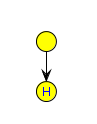
\includegraphics[width=50px]{img/hetero_homo.png}
	\centering
	\caption{El nodo con H contiene un secuente heterog'eneo. El otro nodo es homog'eneo.}
\end{figure}


\subsection{Ramas alternativas}

Para permitir documentar todas las acciones aplicadas as'i como la creaci'on de caminos de an'alisis alternativos introdujimos la noci'on de \textit{ramificaci'on alternativa}.
Las ramas alternativas representan la existencia de m'ultiples caminos en los que se subdivide el an'alisis para lograr un resultado. En la interfaz de usuario de Heterogenius este tipo de ramas se representa con lineas punteadas y su significado sem'antico es el de una disyunci'on. Se corresponde con un camino alternativo en una demostraci'on.

\begin{figure}[htb]
	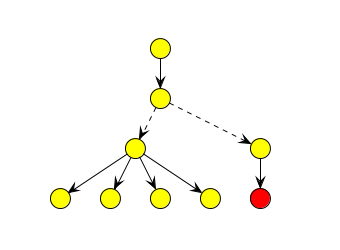
\includegraphics[width=180px]{img/ramas_alternativas_2.png}
	\centering
	\caption{La segunda rama alternativa presenta un contraejemplo. esto indica que existe un contraejemplo para el nodo del cual salen las ramas alternativas.}
        \label{alter1}
\end{figure}

Un nodo con hijos conectados por ramas alternativas se entiende que vale si \textit{\textbf{alguna}} de las ramas valen. Esto es diferente de la ramificaci'on normal (lineas continuas) que indica que el nodo padre vale si todos sus hijos valen.

Al aplicar una ramificaci'on alternativa a un nodo del 'arbol de an'alisis, el nodo es copiado y agregado como sus propios hijos. Esto nos permite trabajar sobre las copias del nodo original. Cuando es necesario tambi'en se puede agregar ramas alternativas durante un an'alisis.
 
La principal ventaja de usar caminos alternativos es la de poder documentar todo el an'alisis que se realiz'o y las decisiones tomadas, incluso las decisiones que no llevaron al cumplimiento del objetivo. Por otro lado tambi'en nos permite experimentar con diferentes formas de probar lo mismo.
En las Fig.~\ref{alter1} y \ref{alter2} se muestran ejemplos de estos usos.

\begin{figure}[bth]
	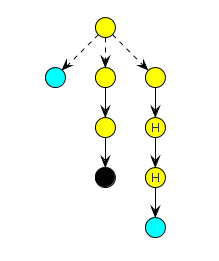
\includegraphics[width=100px]{img/ramas_alternativas.png}
	\centering
	\caption{Tres ramas alternativas: la primera y la 'ultima indican que no se encontr'o ning'un contraejemplo. La segunda rama muestra que se pudo demostrar que el secuente vale, por lo cu'al el secuente del nodo raiz tambi'en vale.}
        \label{alter2}
\end{figure}



\subsection{Nueva Clasificaci'on de Acciones}

Como se ha mencionado, el elemento principal del proceso de demostración en Heterogenius es el 'arbol de an'alisis. All'i es donde se realizan todas las acciones y es donde se refleja el camino tomado para lograr una demostraci'on exitosa. Cada nodo del 'arbol representa un secuente en alg'un lenguaje soportado por Heterogenius. Las aristas se corresponden con las acciones aplicadas a cada secuente. Dependiendo del lenguaje en el que est'e el secuente se habilitan distintas acciones, pero en general se las puede dividir en tres categor'ias:

\begin{description}
\label{clasificacion}
\item[\textbf{reglas del c'alculo de secuentes}:] son acciones que transforman un secuente en otro. Algunas pueden producir múltiples secuentes (por ejemplo la acci'on \emph{Case}) creando varias ramas que tienen que ser demostradas para lograr un resultado en el nodo raiz.

\item[\textbf{traducciones}:] traducen un secuente de un lenguaje a otro. Dependiendo de la expresividad del lenguaje esta traducci'on puede preservar completamente la semántica o sólo parcialmente.

\item[\textbf{búsquedas de contraejemplos}:] implican el uso de herramientas externas para buscar contraejemplos para intentar validar el secuente donde se aplica la acci'on. 
Dependiendo del lenguaje del secuente y del poder de la herramienta seleccionada para realizar la búsqueda, estos procesos pueden verse como análisis parciales ya que podría ser imposible agotar todo el espacio de búsqueda. En tales contextos, una búsqueda infructuosa no brinda mayor información. Por el contrario, la existencia de un contraejemplo es prueba suficiente para saber que la rama en cuestión no podrá ser cerrada.
\end{description}

Si bien esta clasificaci'on serv'ia en la versi'on anterior, debi'o ser modificada para adaptarse a la nueva funcionalidad incluida durante el desarrollo de este trabajo y permitir una mayor flexibilidad a la hora de agregar otras herramientas en el futuro.
La nueva clasificaci'on propuesta se muestra a continuaci'on.

\begin{description}
\item[\textbf{Acciones de c'alculo de secuentes}:] esta categor'ia es ls misma que en la versi'on anterior. Comprende las acciones que permiten avanzar en el an'alisis aplicando reglas del c'alculo de secuentes.

\item[\textbf{Acciones de herramientas estructurales}:] son acciones que trabajan directamente sobre la estructura del 'arbol de an'alisis. Los traductores-$\rho$ forman parte de 'este grupo, asi como las nuevas acciones introducidas: \textit{traducci'on-$\rho$ de f'ormulas} y \textit{proyecci'on de f'ormulas}.

\item[\textbf{Acciones de herramientas automáticas}:] este grupo representa a las acciones para las que se usan herramientas autom'aticas como lo son los demostradores autom'aticos de teoremas y los buscadores de contraejemplos.
\end{description}

Esta clasificaci'on se reflej'o en la arquitectura de Heterogenius y permitir'a guiar las futuras extensiones y funcionalidades adicionales que se deseen implementar.


\newpage
\section{Heterogeneidad Completa}
\label{sec:heterogeneidad-verdadera}

Para ampliar las capacidades de Heterogenius extendimos el concepto de heterogeneidad para lograr tener demostraciones completamente heterog'eneas en lugar de demostraciones heterogéneas pero con secuentes homogéneos. 

La diferencia principal radica en que, con la nueva implementaci'on, los secuentes pueden soportar f'ormulas de diferentes lenguajes. As'i un secuente puede ser de tipo homogéneo o heterogéneo. En el primer caso todas las f'ormulas del secuente usan el mismo lenguaje; en el segundo las f'ormulas son de lenguajes distintos.

La ventaja de los secuentes heterogéneos es que se pueden combinar f'ormulas (lemmas, axiomas) provenientes de distintas especificaciones escritas en lenguajes diferentes. De esta forma nos podemos abstraer del lenguaje en el que están escritas y concentrarnos en el an'alisis.

La principal limitaci'on de los secuentes heterogéneos es que las herramientas (calculadores de secuentes, buscadores de contraejemplos, demostradores autom'aticos) trabajan con secuentes escritos en un solo lenguaje, o sea secuentes homogéneos. Debido a esto se proveen nuevas operaciones para el manejo de f'ormulas dentro de un secuente.

\subsection{Operaciones para el manejo de f'ormulas}

Cada una de las siguientes operaciones puede cambiar o no la heterogeneidad de un secuente.  Dependiendo de los lenguajes de las f'ormulas del resultado, el secuente puede pasar a ser heterogéneo, homogéneo o mantener su tipo. Las nuevas operaciones que permiten disponer de un mayor control sobre la heterogeneidad de los secuentes son:

\begin{itemize}
\item Proyecci'on
\item Introducci'on de antecedentes desde una fuente externa
\item Traducci'on
\end{itemize}

\subsubsection{Proyecci'on}

'Esta operaci'on  permite seleccionar un subconjunto de las f'ormulas que se quiere proyectar sobre el secuente actual y el nuevo secuente se forma a partir de las f'ormulas seleccionadas:

%$$ \alpha_1,\ldots,\alpha_n \vdash \alpha_{n+1},\ldots,\alpha_m $$
%\begin{prooftree}
%\AxiomC{$\alpha_1$,$\ldots$,$\alpha_n$}
%\UnaryInfC{$\alpha_{n+1}$,$\ldots$,$\alpha_m$}
%\end{prooftree}

\begin{prooftree}
\AxiomC{$\{\alpha_{i\in [1,n]\cap\mathcal{C}} \} \vdash \{\alpha_{j\in [n+1, m]\cap\mathcal{C}}\}$}
\RightLabel{Regla de proyecci'on}
\UnaryInfC{$ \alpha_1,\ldots,\alpha_n \vdash \alpha_{n+1},\ldots,\alpha_m $}
\end{prooftree}

con $\mathcal{C} \subseteq \{1 \ldots m\}$, un subconjunto de los 'indices de las f'ormulas que se quieren proyectar.

%\begin{prooftree}
%\AxiomC{$\alpha_i$ con $i=1 \ldots n$ y $i \in \mathcal{C}$}
%\UnaryInfC{$\alpha_j$ con $j=n+1 \ldots m$ y $j \in \mathcal{C}$}
%\end{prooftree}
%$$\{\alpha_i \} \vdash \{\alpha_j\} \mbox{ con }i\in [1,n]\cap\mathcal{C} \mbox{ y } j\in [n+1, m]\cap\mathcal{C}$$
%\vspace{1em}

Si se aplica una operaci'on de proyecci'on a un secuente homog'eneo el resultado siempre ser'a homog'eneo, pero si se empieza con un secuente heterogeneo el resultado puede ser un secuente homog'eneo, si se proyectan f'ormulas de un mismo lenguaje o un secuente heterog'eneo si la proyecci'on incluye f'ormulas de lenguajes diferentes.

A modo de ejemplo, en la Fig.~\ref{seq selection} se muestra el cuadro de di'alogo mediante el cual el usuario puede seleccionar las f'ormulas que se quiere proyectar en el nuevo secuente. Notar que el secuente presentado es heterog'eneo y contiene formulas tanto en \textit{Alloy} como en \textit{TPTP-FOF}.

\begin{figure}[]
	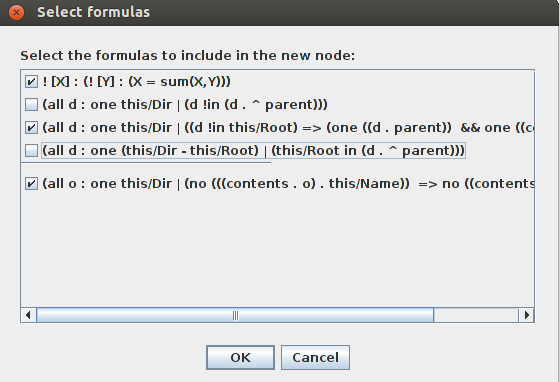
\includegraphics[width=200px]{img/select.png}
	\centering
	\caption{(Cuadro de di'alogo de proyecci'on de f'ormulas)}
        \label{seq selection}
\end{figure}

\subsubsection{Introducci'on de f'ormulas desde una fuente externa}

Esta operaci'on es una generalizaci'on de la regla de corte, que permite cargar f'ormulas desde un archivo de especificaci'on, ya sea escrito en el lenguaje \textit{Alloy} o en \textit{TPTP-FOF}. Al seleccionar las f'ormulas nuevas, se crean dos nodos nuevos que se agregan como hijos del nodo actual. Las f'ormulas a su vez se introducen como hip'otesis en uno de los secuentes y como tesis en el otro.

La operaci'on se puede ejecutar a trav'ez del men'u contextual que se muestra en la Fig. \ref{add antecedents 1}.


\begin{prooftree}
\AxiomC{$ \Gamma,\beta_1,\ldots, \beta_k \vdash \Delta $}
\AxiomC{$ \Gamma\vdash \beta_1,\ldots, \beta_k , \Delta $}
\RightLabel{(Regla de introducci'on de f'ormulas nuevas)}
\BinaryInfC{$ \Gamma \vdash \Delta $}
\end{prooftree}

con $\{\beta_1 \ldots \beta_k\}$ un conjunto de f'ormulas nuevas a introducir.

%\begin{prooftree}
%\AxiomC{$\alpha_1$,$\ldots$,$\alpha_n$}
%\UnaryInfC{$\alpha_{n+1}$,$\ldots$,$\alpha_m$}
%\end{prooftree}
%$$ \alpha_1,\ldots,\alpha_n \vdash \alpha_{n+1},\ldots,\alpha_m $$
%y un conjunto de f'ormulas nuevas $\{\beta_1 \ldots \beta_k\}$. El nuevo secuente es:
%\begin{prooftree}
%\AxiomC{$\alpha_1$,$\ldots$,$\alpha_n,\beta_1,\ldots, \beta_k$}
%\UnaryInfC{$\alpha_{n+1}$,$\ldots$,$\alpha_m$}
%\end{prooftree}
%$$ \alpha_1,\ldots,\alpha_n,\beta_1,\ldots, \beta_k \vdash \alpha_{n+1},\ldots,\alpha_m $$

'Esta operaci'on puede puede conservar o cambiar tanto la homogeneidad como la heterogeneidad del secuente inicial.

\begin{figure}
\centering
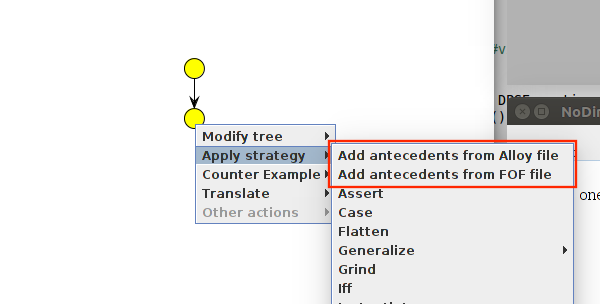
\includegraphics[width=5cm]{img/add_antecedents_1.png}	
\caption{Men'u contextual para seleccionar la fuente de las f'ormulas a introducir.}
\label{add antecedents 1}
\end{figure}


\subsubsection{Traducci'on}

Se extendi'o el concepto de traducciones para que se puedan traducir f'ormulas por separado, en lugar de traducir un secuente completo como en la versi'on anterior.
El secuente resultante contendr'a las f'ormulas del secuente analizado en el lenguaje seleccionado.

\begin{prooftree}
\AxiomC{$ \rho_{\mathcal{T}(\alpha_1)}(\alpha_1) ,\ldots, \rho_{\mathcal{T}(\alpha_n)}(\alpha_n) \vdash \rho_{\mathcal{T}(\alpha_{n+1})}(\alpha_{n+1}) ,\ldots,\rho_{\mathcal{T}(\alpha_m)}(\alpha_m) $}
\RightLabel{(Regla de traducci'on)}
\UnaryInfC{$ \alpha_1,\ldots,\alpha_n \vdash \alpha_{n+1},\ldots,\alpha_m $}
\end{prooftree}

donde $\rho_l$ es la funci'on de traducci'on al lenguaje $L$ y $\mathcal{T}:Formula\rightarrow Lenguaje$ que indica el lenguaje seleccionado para cada f'ormula del secuente original.

%$$ S: \alpha_1,\ldots,\alpha_n \vdash \alpha_{n+1},\ldots,\alpha_m $$
%\begin{prooftree}
%\AxiomC{$\alpha_1$,$\ldots$,$\alpha_n$}
%\UnaryInfC{$\alpha_{n+1}$,$\ldots$,$\alpha_m$}
%\end{prooftree}
%y una función  $\mathcal{T}:Formula\rightarrow Lenguaje$ que indica el lenguaje seleccionado para cada f'ormula del secuente $S$, el secuente resultante es:
%$$ S': \beta_1,\ldots,\beta_n \vdash \beta_{n+1},\ldots,\beta_m $$
%\begin{prooftree}
%\AxiomC{$\beta_1$,$\ldots$,$\beta_n$}
%\UnaryInfC{$\beta_{n+1}$,$\ldots$,$\beta_m$}
%\end{prooftree}


En la Fig. \ref{GUI form translation} se puede ver un cuadro de di'alogo donde el usuario puede seleccionar, para cada f'ormula, el lenguaje al que se quiere traducir.

\begin{figure}[]
	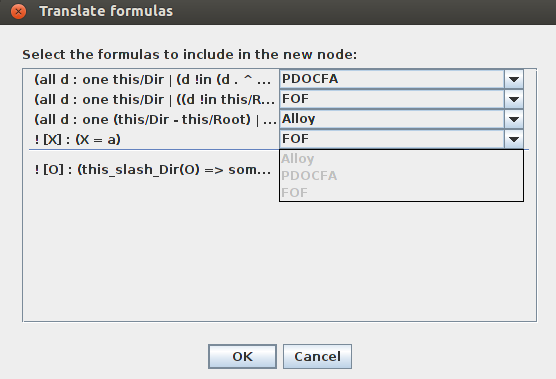
\includegraphics[width=200px]{img/translate.png}
	\centering
	\caption{Cuadro de di'alogo para la traducci'on de f'ormulas en un secuente.} \label{GUI form translation}
\end{figure}



\newpage
\section{Extendiendo Heterogenius con demostradores de primer orden}

Tal como se mencionó en el capítulo \ref{capitulo:TPTP-FOF}, la competencia \textit{CASC} ha adquirido una gran reputación en los últimos años.

Junto a la integraci'on de TPTP-FOF, se incorporaron los siguientes mecanismos para poder usar las herramientas correspondientes.

\begin{itemize}
\item Se permiti'o la carga de especificaciones escritas puramente en TPTP-FOF.

\item Se agreg'o una traducción $\rho$ desde el lenguaje de \textit{PDOCFA} a \textit{TPTP-FOF}. 

\item Se agregaron acciones espec'ificas que permiten invocar a las herramientas en cuesti'on.
\end{itemize}

\subsection{Traducci'on de \emph{PDOCFA} a \emph{TPTP-FOF}}

...\todomm{Esto lo escribo yo}

\todomm{Acá hay que explicar qué es un calculador de secuentes. Y se puede agregar el párrafo que está en el capítulo anterior. La explicación la podés encontrar en el paper de Manu y en su tesis.}

\subsection{Herramientas incorporadas}

Teniendo el soporte de \textit{TPTP-FOF} por parte del motor de c'alculo de secuentes de Heterogenius, integramos algunas de las herramientas mas difundidas en el 'ambito de demostradores autom'aticos de teoremas para el lenguaje \textit{TPTP-FOF}: \textit{SPASS} \cite{WDFKSW09} y \textit{E-Prover} \cite{s13} como calculadores de secuentes y \textit{Mace4} \cite{m05} y \textit{E-Prover} como buscadores de contraejemplos.

\subsubsection{SPASS}

Desde el 2000, tanto \textit{SPASS} como \textit{E-Prover} ocupan los primeros lugares en la competencia anual de demostradores de teoremas \textit{CASC} (CADE ATP System Competition).

\subsection{Modificaciones al c'alculo de Heterogenius}

Al introducir soporte para lenguajes de l'ogica de primer 'orden y herramientas autom'aticas de an'alisis de estos lenguajes, fue necesario tambi'en extender las acciones de demostraci'on de Heterogenius agregando tres reglas nuevas.

Sea $\Gamma \vdash \alpha$ el secuente que se quiere analizar, se introducen las siguientes reglas:

\begin{prooftree}
\LeftLabel{\textbf{Regla 1:}}
\AxiomC{$\top$}
\RightLabel{\qquad si vale $\Gamma \vdash^{fof} \alpha$}
\UnaryInfC{$\Gamma \vdash \alpha$}
\end{prooftree}

Esta regla indica que si se logra encontrar una demostraci'on del secuente $\Gamma \vdash \alpha$ con un demostrador autom'atico de primer orden, la rama se considera cerrada.


\begin{prooftree}
\LeftLabel{\textbf{Regla 2:}}
\AxiomC{$\bot$}
\RightLabel{\qquad si existe $\mathcal{M} \in Mod^{fof}(\Gamma$) y $\mathcal{M} \nvDash^{fof} \alpha$ }
\UnaryInfC{$\Gamma \vdash \alpha$}
\end{prooftree}

Si de lo contrario, se logra encontrar un modelo de $\Gamma$ que no satisface $\alpha$, este modelo es un contraejemplo y la rama contin'ua abierta.


\begin{prooftree}
\LeftLabel{\textbf{Regla 3:}}
\AxiomC{$\Gamma \vdash \alpha$}
\RightLabel{(si no)}
\UnaryInfC{$\Gamma \vdash \alpha$}
\end{prooftree}

Por 'ultimo, debido a que la l'ogica de primer orden no es completa y la ejecuci'on de las herramientas autom'aticas est'a limitada por un \textit{timeout}, es posible no encontrar ni una demostraci'on ni un contraejemplo. En 'este caso no se puede concluir nada y el resultado es el mismo secuente.

Con 'estas reglas se cubren todos los casos, tanto de demostraci'on como los de refutaci'on de una f'ormula de primer 'orden. Al usar alg'un demostrador autom'atico de teoremas se aplican las reglas 1 y 3. En cambio cuando se realiza una b'usqueda de contraejemplo, las reglas usadas son 2 y 3.



TODO: explicar la traduccion PDOCFA -> FOF

\newpage
\section{Detalles de Implementaci'on}

En 'esta secci'on se explicar'an algunas de las dificultades y detalles de las decisiones tomadas al implementar los nuevos conceptos en \textit{Heterogenius}. En particular vamos a explicar la extensi'on de las traducciones $\rho$, la integraci'on del lenguaje \textit{TPTP-FOF} e implementaci'on de buscadores de contraejemplo y demostradores usando las herramientas autom'aticas que trabajan con el lenguaje \textit{TPTP-FOF}.

\subsection{Extensi'on de las traducciones Rho}

\todomm{El punto fuerte de tu trabajo fue la implementación de estos conceptos, así que tenemos que explicar bien esto como para que los jurados lo entiendan así. En principio, deberías explicar un poco cómo estaba diseñado Heterogenius, para que se entienda la magnitud del cambio que realizaste}

Debido a los cambios introducidos fue necesario \textit{refactorizar} el diseño de la infraestructura de las traducciones $\rho$. Lo primero que se hizo fue agregar un \textit{TranslationsManager}, un objeto encargado de manejar todas las traducciones soportadas por el sistema. 

Por otro lado los traductores (subclases de \textit{Translator}) deben implementar los tres m'etodos  abstractos definidos en la clase padre. Cada uno de 'estos m'etodos permite un control m'as fino de las traducciones al separar el secuente en sus partes, que son: una referencia de skolemizac'ion, una especificaci'on y la f'ormula analizada.

\begin{figure}[H]
	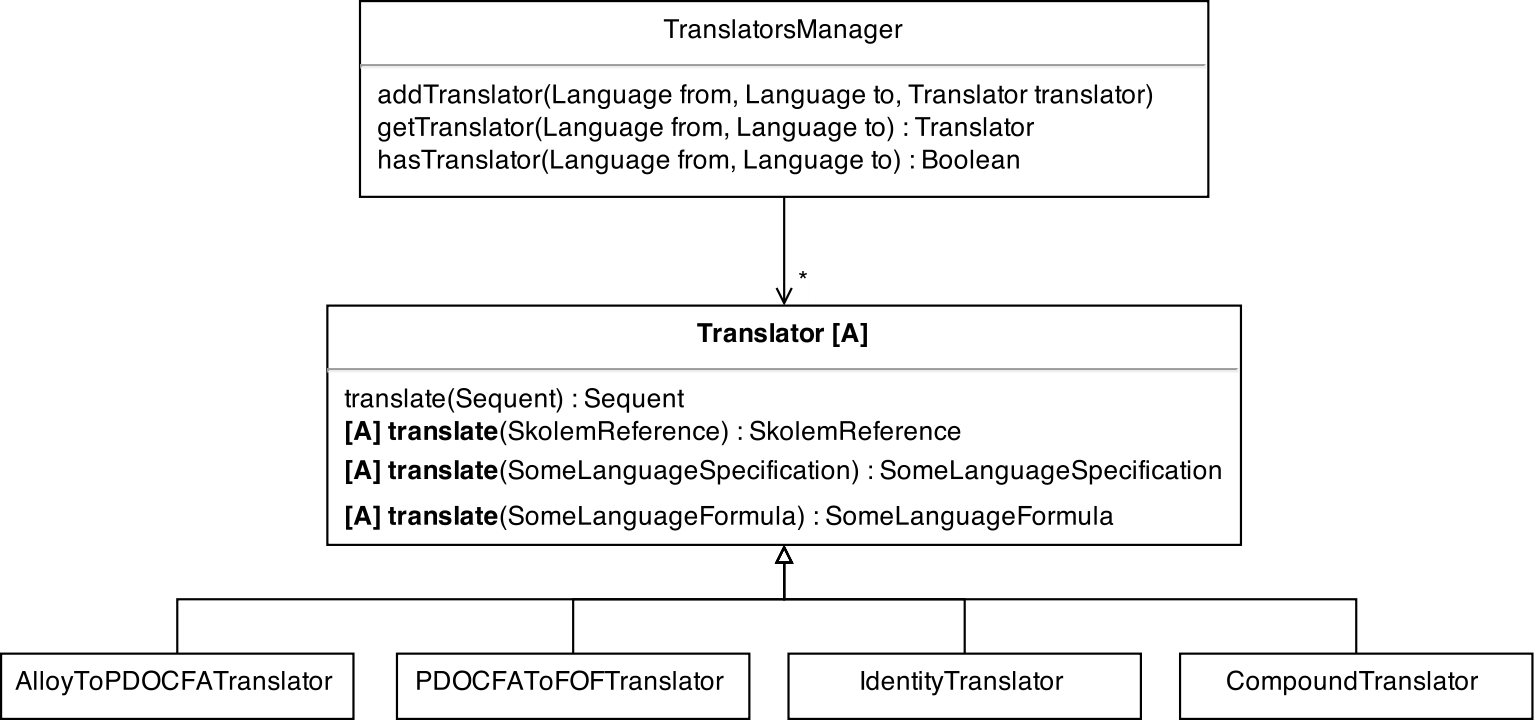
\includegraphics[width=400px, angle=90]{img/arq_traductores.png}
\end{figure}

Se proveen los traductores de \textit{Alloy} a \textit{PDOCFA}, de \textit{PDOCFA} a \textit{TPTP-FOF} asi como el \textit{CompoundTranslator} que permite componer los traductores para lograr traducciones transitivas, por ejemplo de \textit{Alloy} a \textit{TPTP-FOF}.


\subsection{Demostradores de teoremas}

\subsubsection{Preparaci'on del secuente}

El formato \textit{TPTP-FOF} que usan las herramientas autom'aticas agregadas es una lista de f'ormulas escritas en el lenguaje \textit{TPTP-FOF}. Cada una de 'estas f'ormulas debe tener un tipo que puede ser: \textit{axiom} o \textit{conjecture} (existen m'as tipos pero son irrelevantes para nuestro caso).

Para convertir el secuente analizado al formato \textit{TPTP-FOF} se agregan todas las f'ormulas del antecedente con el tipo \textit{axiom} y las f'ormulas del consecuente con el tipo \textit{conjecture}. 

Al ejecutar un demostrador autom'atico con la entrada preparada de este modo, se va a tratar de probar las f'ormulas del consecuente usando que las f'ormulas del antecedente son verdaderas.


\subsubsection{Integraci'on con Heterogenius}

Para integrar las herramientas autom'aticas, tanto los demostradores de teoremas como los buscadores de contraejemplos fue necesario \textit{refactorizar} y extender el diseño de algunas partes de la arquitectura de Heterogenius. Algunos de los objetivos y criterios que se usaron durante el rediseño fueron lograr abstraer las herramientas usadas y hacer un diseño lo suficientemente extensible y abierto para la integraci'on con nuevas herramientas en el futuro.

\begin{figure}[H]
	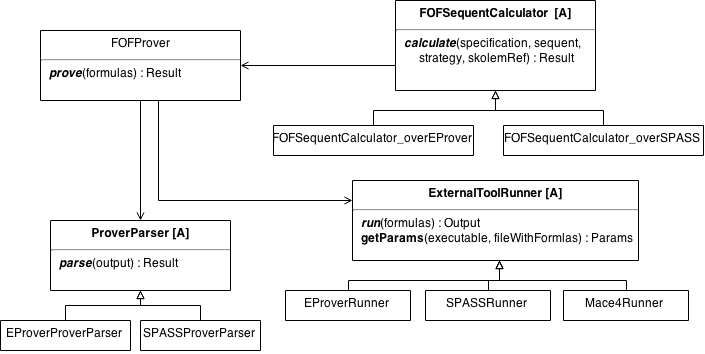
\includegraphics[width=450px, angle=90]{img/arq_prover.png}
	\centering
	\caption{Demostradores autom'aticos usados como calculadores de secuentes.}
\end{figure}

\todomm{Mencionar en la explicación qué roles desempeñan cada una de las entidades mencionadas. Además indicar explícitamente cuáles debieron ser modificadas y cuáles agregadas en la nueva versión.
Para explicar esto podés indicar los pasos que se deberían seguir para incorporar un demostrador nuevo (como lo que está en estos dos párrafos, pero explicado con más detalle).
Y explicar cómo fueron implementados esos pasos para incluir alguno de los demostradores que agregaste.}

Un calculador de secuentes basado en un demostrador autom'atico del lenguaje \textit{TPTP-FOF} se crea subclasificando la clase abstracta \textbf{FOFSequentCalculator}. La nueva clase va a contener un objeto \textit{FOFProver} compuesto con los objetos de las subclases de \textbf{ProverParser} y de \textbf{ExternalToolRunner} correspondientes.

Para agregar una herramienta nueva primero se debe subclasificar la clase abstracta \textbf{ExternalToolRunner}. Esta clase abstrae las particularidades de ejecuci'on de la herramienta especificando los parametros necesarios. Luego se extiende la clase \textbf{ProverParser} que se encarga de procesar el texto correspondiente a la salida de la herramienta. 



\subsection{B'usqueda de contraejemplos}

\subsubsection{Preparaci'on del secuente}

Tanto \textit{Mace4} como \textit{E-Prover} se usan para buscar contraejemplos de los secuentes \textit{TPTP-FOF}. Como las dos herramientas son buscadores de modelos, para preparar el secuente lo que se hace es armar una lista de f'ormulas de tipo \textit{axiom} a partir de las f'ormulas del antecedente y del consecuente del secuente analizado.

Cuando todas las f'ormulas que se envian como entrada a los buscadores de modelos son de tipo \textit{axiom}. Las herramientas tratan de buscar un modelo para el conjunto de los axiomas recibidos.

Lo que se quiere lograr es encontrar un contraejemplo, entonces se hace necesario negar el secuente y buscar un modelo para la negaci'on.

Sea $\{\alpha_1 \dots \alpha_n\} \vdash \{\beta_1 \dots \beta_m\}$ el secuente bajo an'alisis.
La negaci'on se puede escribir como:

\begin{equation}
\bigwedge\limits_{i=1}^n{\alpha_i} \wedge \bigwedge\limits_{j=1}^m{\neg \beta_{j}}
\end{equation}

Con lo cual para armar la lista de f'ormulas de entrada, para cada $\alpha_{i}$ del antecedente se agrega $\alpha_{i}$ como axioma y para cada $\beta_{i}$ del consecuente se agrega $\neg \beta_{i}$ tambi'en como axioma.

Encontrar un modelo para una especificaci'on armada de 'este modo implica la existencia de un contraejemplo para el secuente procesado.


\subsubsection{Integraci'on con Heterogenius}

Tambi'en como en el caso de los demostradores autom'aticos fue necesario \textit{refactorizar} el diseño de los buscadores de contraejemplos para permitir una mayor flexibilidad a la hora de agregar nuevas herramientas con soporte de \textit{TPTP-FOF}.

\begin{figure}[H]
	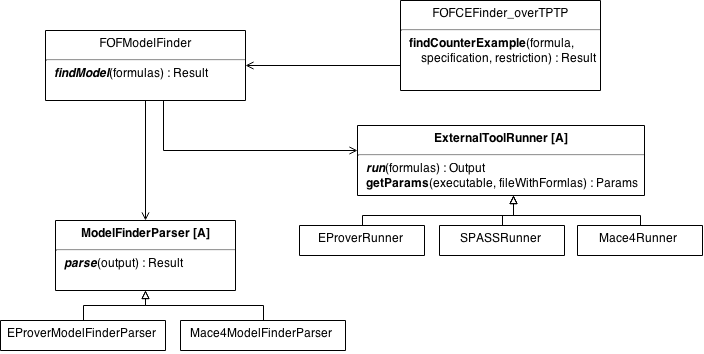
\includegraphics[width=450px, angle=90]{img/arq_ce.png}
	\centering
	\caption{Buscadores de contraejemplos.}
\end{figure}

\todomm{Ídem anterior (a menos que queden demasiado parecidos).}
El diseño de los buscadores de contraejemplos basados en \textit{TPTP-FOF} es an'alogo a los calculadores de secuentes. Se usa la misma clase \textbf{ExternalToolRunner} que en el caso anterior para la abstracci'on de la ejecuci'on de la herramienta en s'i. Pero en lugar de subclasificar \textbf{ProverParser} se subclasifica la clase abstracta \textbf{ModelFinderParser} que tiene un comportamiento an'alogo.


\newpage
\chapter{Caso de Estudio}

\newpage
\chapter{Conclusiones y Trabajos Futuros}

En 'esta tesis se logr'o ampliar algunos conceptos tanto en la teor'ia como en la pr'actica, implementando las mejoras en \textit{Heterogenius}. Primero logramos extender el concepto del 'arbol de an'alisis, implementando ramificaciones alternativas. 'Esto entre otras cosas nos permiti'o crear caminos alternativos en una demostraci'on para analizar diferentes formas de resolver el problema y adem'as mantener el historial de todo el an'alisis en el 'arbol al maneter las ramas que no llevan a un resultado exitoso.

Tambi'en se ampli'o el concepto de heterogeneidad al permitir soportar secuentes heterogeneos. De 'este forma el an'alisis se volvi'o m'as sencillo al introducir un mayor nivel de abstracci'on sobre los lenguajes aceptados por el sistema. Adem'as se incorporaron herramientas y acciones para traducir, seleccionar o combinar las f'ormulas dentro de un secuente dado.

Luego se extendi'o la funcionalidad de \textit{Heterogenius} con el lenguaje de l'ogica de primer 'orden \textit{TPTP-FOF} y algunas herramientas autom'aticas que trabajan con dicho lenguaje. En particular se integraron dos demostradores autom'aticos de teoremas: \textit{EProver} y \textit{SPASS} y dos buscadores de modelos finitos: \textit{EProver} y \textit{Mace4}. Para que 'esta integraci'on fuera posible fue necesario definir una traducci'on desde el lenguaje \textit{PDOCFA} a \textit{TPTP-FOF}, tomando en cuenta las diferencias de expresividad entre los dos lenguajes.

Por 'ultimo se evaluaron las herramientas autom'aticas integradas sobre un conjunto de lemas de XXX, mostrando cuales son los casos donde 'estas herramientas logran mejores o peores resultados.

'Esta tesis abre varias posibilidades para la extensi'on de \textit{Heterogenius} con m'as herramientas que soporten el lenguaje \textit{TPTP-FOF}. Tambi'en al haber realizado un refactoreo del c'odigo se brinda un mayor soporte de extensi'on para nuevos lenguajes como por ejemplo \textit{TPTP-HOL} un lenguaje de l'ogica de alto 'orden, lenguajes que trabajen sobre l'ogicas temporales, etc.

Con lo cu'al algunas de las mejoras y aportes que se pueden realizar son:

\begin{itemize}

\item Mejorar la interfaz y la interacci'on con el usuario, permitiendo una mayor facilidad de uso de la herramienta.

\item Extender \textit{Heterogenius} con lenguajes y herramientas autom'aticas nuevas.

\item Implementar las acciones de c'alculo de secuentes para el lenguaje \textit{TPTP-FOF} para permitir analisis y demostraciones completas en 'este lenguaje.

\item Agregar herramientas autom'aticas que trabajen con las l'ogicas relacionales para solucionar los problemas mostrados en \ref{analisis_lemas}.

\end{itemize}



%á

%\newpage

\begin{thebibliography}{tesis}

\bibitem{tptp}
	Sutcliffe, G. The TPTP Problem Library and Associated Infrastructure: The FOF and CNF Parts, v3.5.0. Journal of Automated Reasoning. Vol. 43. Num. 4. Pp. 337-362. 2009.

\bibitem{casc}
	The CADE ATP System Competition
	\url{http://www.cs.miami.edu/~tptp/CASC/}

\bibitem{fof}
	FOF: First Order Formula
	\url{http://www.cs.miami.edu/~tptp/TPTP/SyntaxBNF.html}

\bibitem{heterogenius}
	Manuel Gimenez, Mariano Miguel Moscato, Carlos G. Lopez Pombo, and Marcelo F. Frias. Heterogenius: a framework for hybrid analysis of heterogeneous software specifications. In Aguirre and Ribeiro \cite{AR13}, pages 1045–1058. Workshop affiliated to \cite{DM13}. 2013.
	
\bibitem{m05}
	McCune, W., "Prover9 and Mace4", http://www.cs.unm.edu/~mccune/Prover9, 2005-2010. 

\bibitem{s13}
  Schulz, S. System Description: E 1.8, Proceedings of the 19th LPAR, Stellenbosch, 2013, pp. 477-483, LNCS 8312 © Springer Verlag.

\bibitem{WDFKSW09} Weidenbach C., Dimova D., Fietzke A., Kumar R., Suda M. and Wischnewski P., 2009, SPASS Version 3.5. in 22nd International Conference on Automated Deduction, CADE 2009, LNCS 5663, pp. 140-145.

\bibitem{BRJ98} Grady Booch, Jim Rumbaugh, and Ivar Jacobson. The unified modeling language user guide. Addison–Wesley Longman Publishing Co., Inc., Boston, MA, USA, 1998.

\bibitem{Pnu77} Amir Pnueli. The temporal logic of programs. In Proceedings of 18th. Annual IEEE Symposium on Foundations of Computer Science \cite{IEE77}, pages 46–57. 

\bibitem{IEE77} IEEE Computer Society. 18th. Annual IEEE Symposium on Foundations of Computer Science, Los Alamitos, CA, USA, 1977. IEEE Computer Society. 

\bibitem{MP95} Zohar Manna and Amir Pnueli. Temporal Verification of Reactive Systems. Springer-Verlag, New York, 1995. 

\bibitem{HKT00} David Harel, Dexter Kozen, and J. Tiuryn. Dynamic logic. Foundations of Computing. MIT Press, Cambridge, MA, USA, 2000.  

\bibitem{GB84} Joseph A. Goguen and Rod M. Burstall. Introducing institutions. In Clarke and Kozen \cite{CK84}, pages 221–256.  

\bibitem{CK84} Edmund M. Clarke and Dexter Kozen, editors. Carnegie Mellon Workshop on Logic of Programs, volume 184 of Lecture Notes in Computer Science. Springer-Verlag, 1984. 

\bibitem{GB92} Joseph A. Goguen and Rod M. Burstall. Institutions: abstract model theory for specification and programming. Journal of the ACM, 39(1):95–146, 1992. 

\bibitem{Tar96} Andrzej Tarlecki. Moving between logical systems. In Haveraaen et al. \cite{HOD96}, pages 478–502.

\bibitem{HOD96} Magne Haveraaen, Olaf Owe, and Ole-Johan Dahl, editors. Selected papers from the 11th Workshop on Specification of Abstract Data Types, joint with the 8th COMPASS Workshop on Recent

\bibitem{Dia02} Razvan Diaconescu. Grothendieck institutions. Applied Categorical Structures, 10(4):383–402, 2002.

\bibitem{NE02} Mogens Nielsen and Uffe Engberg, editors. International Con- ference on Foundations of Software Science and Computation Structures, Lecture Notes in Computer Science, London, UK, 2002. Springer-Verlag.

\bibitem{Mos02} Till Mossakowski. Heterogeneous development graphs and heterogeneous borrowing. In Nielsen and Engberg \cite{NE02}, pages 326–341. 

\bibitem{DF96} Razvan Diaconescu and Kokichi Futatsugi. Logical semantics for CafeOBJ. Technical Report JAIST-IS-RR-96-0024S, Japan Advanced Institute of Science and Technology, 1996. 

\bibitem{DF02} Razvan Diaconescu and Kokichi Futatsugi. Logical foundations of CafeOBJ. Theoretical Computer Science, 285(2):289–318, 2002. 

\bibitem{JV06}  Michael Johnson and Varmo Vene, editors. 11th. International Conference on Algebraic Methodology and Software Technology, AMAST 2006, volume 4019 of Lecture Notes in Computer Science, Kuressaare, Estonia, July, 5–8 2006. Springer-Verlag. 

\bibitem{LF06} Carlos G. Lopez Pombo and Marcelo F. Frias. Fork algebras as a sufficiently rich universal institution. In Johnson and Vene \cite{JV06}, pages 235–247. 

\bibitem{AR13} Nazareno M. Aguirre and Leila Ribeiro, editors. Latin American Workshop on Formal Methods 2013, August 2013. Workshop affiliated to \cite{DM13}. 

\bibitem{DM13} Pedro R. D’Argenio and Hernán Melgratti, editors. 24th International Conference on Concurrency Theory – CONCUR 2013, volume 8052 of Lecture Notes in Computer Science. Springer- Verlag, 2013.

\bibitem[FBL01]{frias:relmics01}
Marcelo~{F.} Frias, Gabriel~{A.} Baum, and Carlos~{G.} {Lopez Pombo}.
\newblock A comparisson of $\mathbf{A_g}$ with {Alloy}.
\newblock In de~Swart \cite{relmics01}, pages 365--377.

\bibitem[dS01]{relmics01}
Harrie de~Swart, editor.
\newblock {\em 6th. Conference on Relational Methods in Computer Science
  ({RelMiCS}) - {TARSKI}}, Oisterwijk, The Netherlands, October 2001.
  
\bibitem{goguen:cmwlp84}
	Joseph A. Goguen and Rod M. Burstall. Introducing institutions. In Edmund M. Clarke and Dexter Kozen, editors, Proceedings of the Carnegie Mellon Workshop on Logic of Programs, volume 184 of Lecture Notes in Computer Science, pages 221–256. Springer-Verlag, 1984.

\bibitem{goguen:jacm-39_1}
  Joseph A. Goguen and Rod M. Burstall. Institutions: abstract model theory for specification and programming. Journal of the ACM, 39(1):95–146, 1992.

\bibitem{meseguer:lc87}
	Jos'e Meseguer. General logics. In Heinz-Dieter Ebbinghaus, Jos'e Fernandez-Prida, Manuel Garrido, Daniel Lascar, and Mario Rodr'ıguez Artalejo, editors, Proceedings of the Logic Colloquium ’87, volume 129, pages 275–329, Granada, Spain, 1989. North Holland.

\bibitem{tarlecki:sadt-rtdts95}
	Andrzej Tarlecki. Moving between logical systems. In Magne Have- raaen, Olaf Owe, and Ole-Johan Dahl, editors, Selected papers from the 11th Workshop on Specification of Abstract Data Types Joint with the 8th COMPASS Workshop on Recent Trends in Data Type Specification, volume 1130 of Lecture Notes in Computer Science, pages 478–502. Springer-Verlag, 1996.

\bibitem{borzyszkowski:tcs-286_2}
	Tomasz Borzyszkowski. Logical systems for structured specifications. Theoretical Computer Science, 286:197–245, 2002.

\bibitem{gentzen1935}
	G. Gentzen. Untersuchungen uber das logische schließen i. I. Mathema- tische zeitschrift 39, pages 176–210, 1935.
	
\bibitem{bookFoundations}
	Jean H. Gallier. Logic For Computer Science: Foundations of Automatic Theorem Proving. Wiley, 2003.

\bibitem[Fri02]{frias02}
Marcelo~{F.} Frias.
\newblock {\em Fork algebras in algebra, logic and computer science}, volume~2
  of {\em Advances in logic}.
\newblock World Scientific Publishing Co., Singapore, 2002.

\end{thebibliography}




%%%% BIBLIOGRAFIA
%\backmatter
%\bibliography{tesis}

\end{document}

%á
